\section{Técnicas de clasificación contextualizadas}
En este capítulo comentaremos distintos experimentos de clasificación realizados en base al dataset anotado en el capítulo anterior.


\subsection{Trabajos previos}

Como contamos en la anterior sección, son pocos los trabajos y datasets que poseen contexto. Ver \ref{sec:dataset_trabajos_previos} para un repaso de los distintos datasets contextualizados.

\citet{gao2018detecting} propone dos tipos de modelos: regresiones logísticas y redes neuronales recurrentes. Para los modelos de regresiones logísticas, usan como inputs bolsas de palabras, bolsas de caracteres, vectores semánticos producidos con Linguistic Inquiry and Word Count (LIWC) \cite{pennebaker2001linguistic} y features de un lexicon de emociones \cite{mohammad2013nrc}. Por otro lado, utiliza LSTM bidireccionales con mecanismo de atención de Bahdanau \cite{bahdanau2014neural} usando embeddings \emph{word2Vec} de dimensión 100.

Un punto criticable de este trabajo es que utiliza el nombre de usuario como feature; algo que a priori no suele hacerse ya que permitiría ``prejuzgar'' a un usuario antes que por el contenido de sus tweets. Si bien es cierto que la información de usuarios y sus conexiones es valiosa, introducir esta información a nuestros modelos da lugar a posibles correlaciones espurias que es preferible evitar.

\subsection{Tareas de clasificación propuestas}

Now that we have this specially-crafted corpus containing context, we now turn our attention to answer our original question: can classifiers leverage context to improve their performance on the hate speech detection task?

For this purpose, we propose the following classification tasks:

\begin{enumerate}
    \item Task A: Given a tweet, predict whether it is hateful or not
    \item Task B: Given a hateful tweet, predict whether it calls to action and predict the offended characteristics
\end{enumerate}

Each instance consists of both the comment (the tweet) and its context (both title and the full body). To test our hypothesis, for each task we trained classifiers having as input the following comibinations:

\begin{enumerate}
    \item The comment
    \item The title and the comment
    \item The title, the body and the comment
\end{enumerate}


\subsection{Cotas a la performance}

\begin{table}
    \centering
    \begin{tabular}{lll|ll}
        \hline
                   & \multicolumn{2}{c}{Entre anotadores} & \multicolumn{2}{c}{Contra gold} \\
        {}         &  F1 mean&  F1 median  & F1 Mean  &  F1 Median \\
        \hline
        HATEFUL    &  0.6525 &   0.6751    & 0.8285   &   0.8515   \\
        CALLS      &  0.6042 &   0.7037    & 0.7741   &   0.9148   \\
        WOMEN      &  0.7258 &   0.7368    & 0.8371   &   0.8275   \\
        LGBTI      &  0.8939 &   0.9600    & 0.9660   &   0.9743   \\
        RACISM     &  0.9458 &   0.9592    & 0.9667   &   0.9731   \\
        CLASS      &  0.7310 &   0.7500    & 0.8058   &   0.8391   \\
        POLITICS   &  0.7370 &   0.7777    & 0.8920   &   0.9189   \\
        DISABLED   &  0.7973 &   0.8800    & 0.8976   &   0.9392   \\
        APPEARANCE &  0.8033 &   0.9024    & 0.9026   &   0.9493   \\
        CRIMINAL   &  0.8180 &   0.9473    & 0.9614   &   0.9788   \\
        \hline
    \end{tabular}
    \caption{Estadísticos de los cálculos de F1 entre anotadores - modo jerárquico}
    \label{tab:ia_f1_scores}
\end{table}

Como observamos en la anterior sección, la tarea de detección de lenguaje discriminatorio contiene una alta cantidad de ruido, y el acuerdo entre humanos es moderado. En este contexto, cabe preguntarse cuál es la máxima performance que puede lograr un clasificador para esta tarea. Por la misma naturaleza del problema, claramente no puede ser perfecta.

Para obtener algunas medidas de esto, calculamos en primer lugar las F1 usando todos los posibles pares de anotadores. Como la F1 es simétrica (invirtiendo roles se invierten la precisión y la sensibilidad) no necesitamos hacer ninguna asunción sobre cuál sus roles.

Algo a tener en cuenta es que nuestra métrica final será contra la etiqueta resultante del (nuestro \emph{gold standard}). Una cota que seguro está por arriba de nuestra performance es el acuerdo que haya entre los anotadores y este \emph{gold standard}; hay que también observar que cada etiqueta ``de oro'' codifica información de sus anotaciones, con lo cual éste número es una cota superior sin dudas pero también pueden ser demasiado ``gruesa''.

La tabla \ref{tab:ia_f1_scores} contiene estadísticos de estos cálculos, tanto entre anotadores como contra el \emph{gold-standard}. Como podemos observar, la mediana entre anotadores de la F1 (usada para obviar outliers) es relativamente baja para la detección de odio ($\sim 0.67$), mientras que contra el gold standard es de $0.85$. De esto entendemos que la performance máxima en la detección está entre esos dos números.

Por otro lado, para el resto de las características observamos números más elevados, pero hay que recordar que estos cálculos están hecho \textbf{solamente} entre tweets etiquetados como odiosos. Si obviamos esta restricción (lo que llamamos ``modo libre''), la performance esperada baja sustancialmente. La tabla \ref{tab:ia_f1_scores_free_mode} muestra estos números, tanto calculado entre anotadores como contra el \emph{gold standard}.

\begin{table}
    \centering
    \begin{tabular}{lll|ll}
        \hline
                   & \multicolumn{2}{c}{Entre anotadores} & \multicolumn{2}{c}{Contra gold} \\
        {}         &  F1 mean&  F1 median  & F1 Mean  &  F1 Median \\
        \hline
        CALLS      &  0.4341 &   0.4950   &  0.7042   &   0.8424  \\
        WOMEN      &  0.4896 &   0.4676   &  0.7406   &   0.7593  \\
        LGBTI      &  0.5959 &   0.5765   &  0.8462   &   0.9152  \\
        RACISM     &  0.6532 &   0.6444   &  0.8712   &   0.8789  \\
        CLASS      &  0.4431 &   0.4444   &  0.7220   &   0.7317  \\
        POLITICS   &  0.4609 &   0.4360   &  0.7951   &   0.8155  \\
        DISABLED   &  0.5502 &   0.6000   &  0.8127   &   0.8421  \\
        APPEARANCE &  0.6485 &   0.7428   &  0.8314   &   0.9146  \\
        CRIMINAL   &  0.5265 &   0.5801   &  0.8415   &   0.9292  \\
        \bottomrule
    \end{tabular}

    \caption{Estadísticos de los cálculos de F1 entre anotadores - modo libre. Cada característica es tomada como una etiqueta binaria independientemente del cálculo de odio}
    \label{tab:ia_f1_scores_free_mode}
\end{table}


\subsection{Preprocessing}

Para cada tweet, aplicamos el siguiente procesamiento previo: primero, cortamos las repeticiones de caracteres hasta tres ocurrencias; risas normalizadas; los identificadores de usuario (\emph{@user}) se reemplazan por un token especial \emph{[USER]}; convertimos emojis en una representación de texto usando la biblioteca de python \emph{emoji} \footnote {\url{https://github.com/carpedm20/emoji/}}. Los hashtags se eliminan, están rodeados por una ficha especial \emph{[HASHTAG]} y se dividen en palabras si están en mayúsculas.

Aunque no realizamos un análisis de ablación para evaluar el impacto de cada paso del preprocesamiento, el proceso general pareció mejorar el rendimiento de la clasificación en el conjunto de datos de desarrollo.

\subsection{Clasificadores}

Los clasificadores propuestos se basan en \emph{BETO}\cite{canete2020spanish}, una versión en español de \emph{BERT} \cite{devlin2018bert}. \emph{BETO} tiene un tamaño similar a \emph {BERT Base}, y tiene 12 capas de transformadores con 12 cabezas de atención cada una, sumando 110 millones de parámetros. Para obtener más referencias sobre arquitecturas BERT y Transformer, sugerimos CITA NECESARIA.

Para la tarea de detección del discurso de odio, presentamos versiones sin contexto y conscientes del contexto, utilizando el título y el cuerpo completo como posibles contextos. Usamos el token especial BERT \emph {[SEP]} para codificar el contexto y el texto analizado. Recuerde que el token \emph {[SEP]} se usa para la tarea de predicción de la siguiente oración (tarea NSP) en el preentrenamiento al estilo BERT.

En cuanto a la detección de características ofendidas, consideramos este problema como una tarea de clasificación multibinaria; es decir, dado un texto odioso y una característica protegida, lo consideramos como una tarea de clasificación binaria para predecir si el texto ofende la característica respectiva. En lugar de entrenar un clasificador diferente para cada característica, entrenamos un BERT de múltiples salidas, compartiendo todos sus pesos con la excepción de 9 capas lineales diferentes para cada salida. La pérdida utilizada es

\begin{equation*}
    J = \sum\limits_{c \in CHAR \cup \{CALLS\}} J_c
\end{equation*}

donde $CHAR$ es el conjunto de todas las características protegidas (MUJERES, LGBTI, RACISMO, CLASE, etc.) y $CALLS$ es `` llamadas a la acción ''. $ J_c $, ya que cualquier $ c $ es una pérdida de entropía cruzada binaria.

Para tener costos computacionales más amigables, limitamos nuestras secuencias a 128, 256 y 512 tokens para el modelo no contextualizado, el modelo de título y el modelo de título y cuerpo, respectivamente.


\section{Resultados}


\begin{table*}[ht!]
    \centering
    \begin{tabular}{lllll}
        \toprule
        Model &          Precision &             Recall &                 F1 &           Macro F1 \\
        \midrule
        BERT No Context &  $0.682 \pm 0.020$ &  $0.593 \pm 0.018$ &  $0.634 \pm 0.006$ &  $0.785 \pm 0.003$ \\
        BERT Title      &  $0.751 \pm 0.012$ &  $0.603 \pm 0.011$ &  $0.669 \pm 0.007$ &  $0.807 \pm 0.004$ \\
        BERT Title+Body &  $0.738 \pm 0.008$ &  $0.616 \pm 0.005$ &  $0.671 \pm 0.004$ &  $0.808 \pm 0.002$ \\
        \bottomrule
    \end{tabular}


    \caption{Task A: Hate speech detection classification results. Each row contains the performance of the models in complexity order: from the model having no context to the model having full context (title and body). }
    \label{tab:task_a_results}
\end{table*}


La tabla \ref{tab:task_a_results} contiene los resultados de la clasificación, medidos por precisión, recuperación, F1 y Macro F1 (como se acostumbra en algunas tomas compartidas de Detección de discurso de odio y lenguaje ofensivo). Podemos observar que agregar contextos parece mejorar el desempeño; en particular, el simple hecho de agregar el título parece proporcionar suficiente contexto para la tarea de detección del discurso de odio. Agregar el cuerpo mejora marginalmente el rendimiento, pero a un costo computacional más alto (recuerde que la longitud máxima con título se establece en 256, y en el otro caso es 512). La mejora en la puntuación de F1 con solo agregar el título es de aproximadamente 3 puntos; título y cuerpo suma alrededor de 3,5 puntos F1 sobre la clasificación no contextualizada. Al analizar los modelos contextuales, el cuerpo completo parece mejorar el recuerdo al tiempo que disminuye ligeramente la precisión, con una puntuación general igual de F1 que el modelo de solo título.

\begin{figure*}[t]
    \centering
    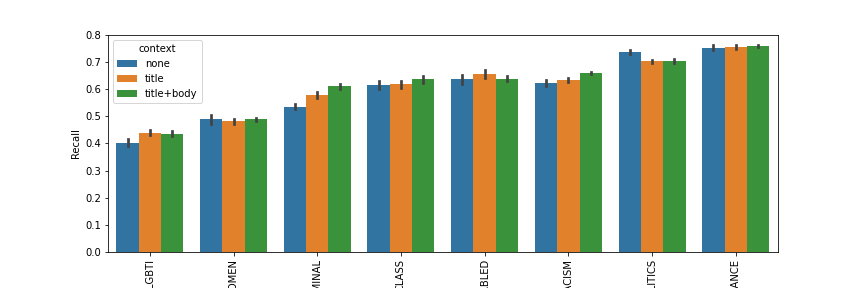
\includegraphics[width=\textwidth]{img/recall_category.png}
    \caption{Recall by characteristic for each model}
    \label{fig:recall_by_characteristic}
\end{figure*}

La figura \ref{fig:recall_by_characteristic} muestra la recuperación de nuestros algoritmos. Usar solo el contexto del título mejora la sensibilidad para las características LGBTI y CRIMINALES (Mann Whitney U, $ p \ leq 0.01 $, Bonferroni corregido); agregar el cuerpo completo también lo mejora significativamente para la característica RACISMO y lo mejora un poco más para CRIMINAL (Mann Whitney U $ p \ leq 0.01 $, Bonferroni corregido). Sin embargo, el desempeño en POLÍTICA empeora al agregar contexto en cualquier forma ($ p \ leq 0.001 $, corregido Bonferroni). Para las otras características, el contexto no mejora ni empeora el desempeño.


% \begin{table}
%     \centering
%     \begin{tabular}{ll}
%         \toprule
%         Model &            Mean F1 \\
%         \midrule
%         BERT No Context &  $0.731 \pm 0.004$ \\
%         BERT Title      &  $0.808 \pm 0.006$ \\
%         BERT Title+Body &  $0.824 \pm 0.006$ \\
%         \bottomrule
%     \end{tabular}
%     \caption{Mean F1 scores for Task B: Offended characteristic detection}
%     \label{tab:task_b_results}
% \end{table}

La figura \ref{fig:task_b_results} muestra los resultados de la característica ofendida y la tarea de detección de llamada a la acción. La tabla \ref{tab:task_b_results} muestra las puntuaciones F1 medias para tener una medida de resumen. Como se esperaba, la ganancia de tener contexto disponible es más evidente en este punto, con una diferencia media de puntuación F1 de $ 7,6 $ puntos entre no tener contexto y tener el título, y $ 1,5 $ puntos adicionales si el cuerpo está disponible. La detección de llamadas a la acción apenas se mejora al tener un contexto disponible. Nuevamente, las características LGBTI y CRIMINALES se benefician enormemente del contexto; La característica CLASS también parece tener alguna mejora. No hay grandes diferencias entre tener el título y el cuerpo completo.

\begin{figure*}[t]
    \centering
    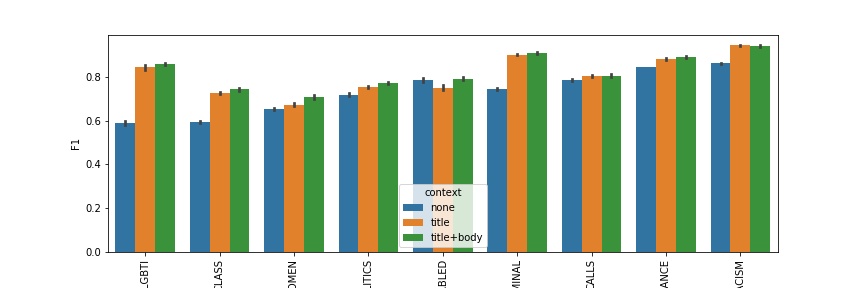
\includegraphics[width=\textwidth]{img/task_b_scores.png}
    \caption{F1 scores for each characteristic in Task B: offended characteristic detection}
    \label{fig:task_b_results}
\end{figure*}

\begin{table*}
    \centering
    \begin{tabular}{llll}
        \toprule
        {} &    BERT No Context &         BERT Title &    BERT Title+Body \\
        \midrule
        Calls F1       &  $0.784 \pm 0.009$ &  $0.802 \pm 0.010$ &  $0.805 \pm 0.017$ \\
        Women F1       &  $0.652 \pm 0.011$ &  $0.672 \pm 0.015$ &  $0.708 \pm 0.017$ \\
        Lgbti F1       &  $0.590 \pm 0.018$ &  $0.843 \pm 0.021$ &  $0.857 \pm 0.012$ \\
        Racism F1      &  $0.863 \pm 0.005$ &  $0.943 \pm 0.004$ &  $0.939 \pm 0.007$ \\
        Class F1       &  $0.593 \pm 0.011$ &  $0.727 \pm 0.012$ &  $0.742 \pm 0.014$ \\
        Politics F1    &  $0.718 \pm 0.015$ &  $0.753 \pm 0.007$ &  $0.771 \pm 0.012$ \\
        Disabled F1    &  $0.786 \pm 0.016$ &  $0.750 \pm 0.029$ &  $0.791 \pm 0.015$ \\
        Appearance F1  &  $0.845 \pm 0.004$ &  $0.879 \pm 0.010$ &  $0.892 \pm 0.010$ \\
        Criminal F1    &  $0.744 \pm 0.009$ &  $0.901 \pm 0.008$ &  $0.907 \pm 0.008$ \\
        \hline
        Mean F1        &  $0.731 \pm 0.004$ &  $0.808 \pm 0.006$ &  $0.824 \pm 0.006$ \\
        Mean Precision &  $0.786 \pm 0.004$ &  $0.853 \pm 0.007$ &  $0.851 \pm 0.006$ \\
        Mean Recall    &  $0.687 \pm 0.006$ &  $0.770 \pm 0.008$ &  $0.800 \pm 0.007$ \\
        \bottomrule
    \end{tabular}
    \caption{Performance of models for Task B: offended characteristic detection. Mean and standard deviation for 15 runs are displayed. }
    \label{tab:task_b_results}
\end{table*}


\section{Análisis de error}

\section{Discusión}

Para esta tarea en particular, podemos observar que el contexto parece dar una mejora moderada en la tarea de detección del discurso de odio (alrededor de 3 puntos F1), ninguna mejora significativa en la detección de llamadas a la acción, y una mejora considerable en la tarea característica ofendida (alrededor de 7 puntos F1 medios).

Si bien este resultado podría estar en aparente contradicción con un trabajo reciente que no encontró ninguna mejora mediante el contexto en la detección de toxicidad \cite{pavlopoulos2020toxicity}, se puede señalar que la detección del discurso de odio es una de las formas más complejas de ``tóxico'' comportamiento y, como tal, podría permitir que los clasificadores tengan más información para predecir si el texto dado es odioso o no. Otra razón detrás de este resultado es el dominio de nuestro conjunto de datos: mientras que \citet{pavlopoulos2020toxicity} usa el contexto conversacional, nosotros usamos el título y el cuerpo del artículo como contexto para los comentarios de los usuarios.

Este trabajo tiene algunas limitaciones. Primero, una consideración práctica es que no siempre tenemos un contexto disponible para un texto dado. Incluso si podemos encontrarlo, a veces este contexto puede no ser en forma de artículo de noticias, sino como un hilo de conversación o incluso de alguna otra forma (¿una base de conocimiento?).

\section{Limitaciones y trabajo futuro}